Для установившегося режима фильтрации давление в пласте не меняется. Для псевдо-установившегося режима постоянным остается перепад давления между пластом и забоем. После запуска, остановки или изменения режима работы скважины эти условия не выполняются. Давление в различных точках пласта может меняться по разному. Такой режим называют неустановившимся, а решения его описывающие нестационарными (зависят от времени).

Неустановившиеся решения уравнения фильтрации (transient solutions) представляют значительный практический интерес во многих задачах, включая задачи интерпретации ГДИС. В тоже время они относительно сложны и требуют применения компьютерных алгоритмов. В данном пособие проведение расчетов иллюстрируется с использованием макросов для Excel -- Unifloc VBA.

\section{Решение линейного стока}

Для решения уравнения фильтрации - линейного дифференциального уравнения в частных производных второго порядка необходимо задать начальные и граничные условия. 

Самое простое решение можно получить для случая вертикальной скважины бесконечно малого радиуса запускающейся с постоянным дебитом. Условия соответствующие этому случаю можно выразить следующим образом:

\begin{itemize}
	\item Начальное условие. До запуска скважины в момент времени  $t_D = 0$ давление в пласте равно начальному во всех точках $p=p_i$
	$$ t_D < 0, p_D = 0 $$ 
	\item Граничное условие на скважине.  Условие постоянства дебита на скважине можно трансформировать в граничное условие опираясь на закон Дарси.
	$$ \lim_{r_D \to 0} {r_D \frac{\partial p_D}{\partial r_D}} = -1$$
	\item Граничное условие на бесконечном расстоянии от скважины. Давление в пласте на бесконечно большом расстоянии от скважины равно начальному.
	$$ r_D = \infty, p_D = 0$$
\end{itemize}

\begin{figure}[h!]
	\begin{center}
		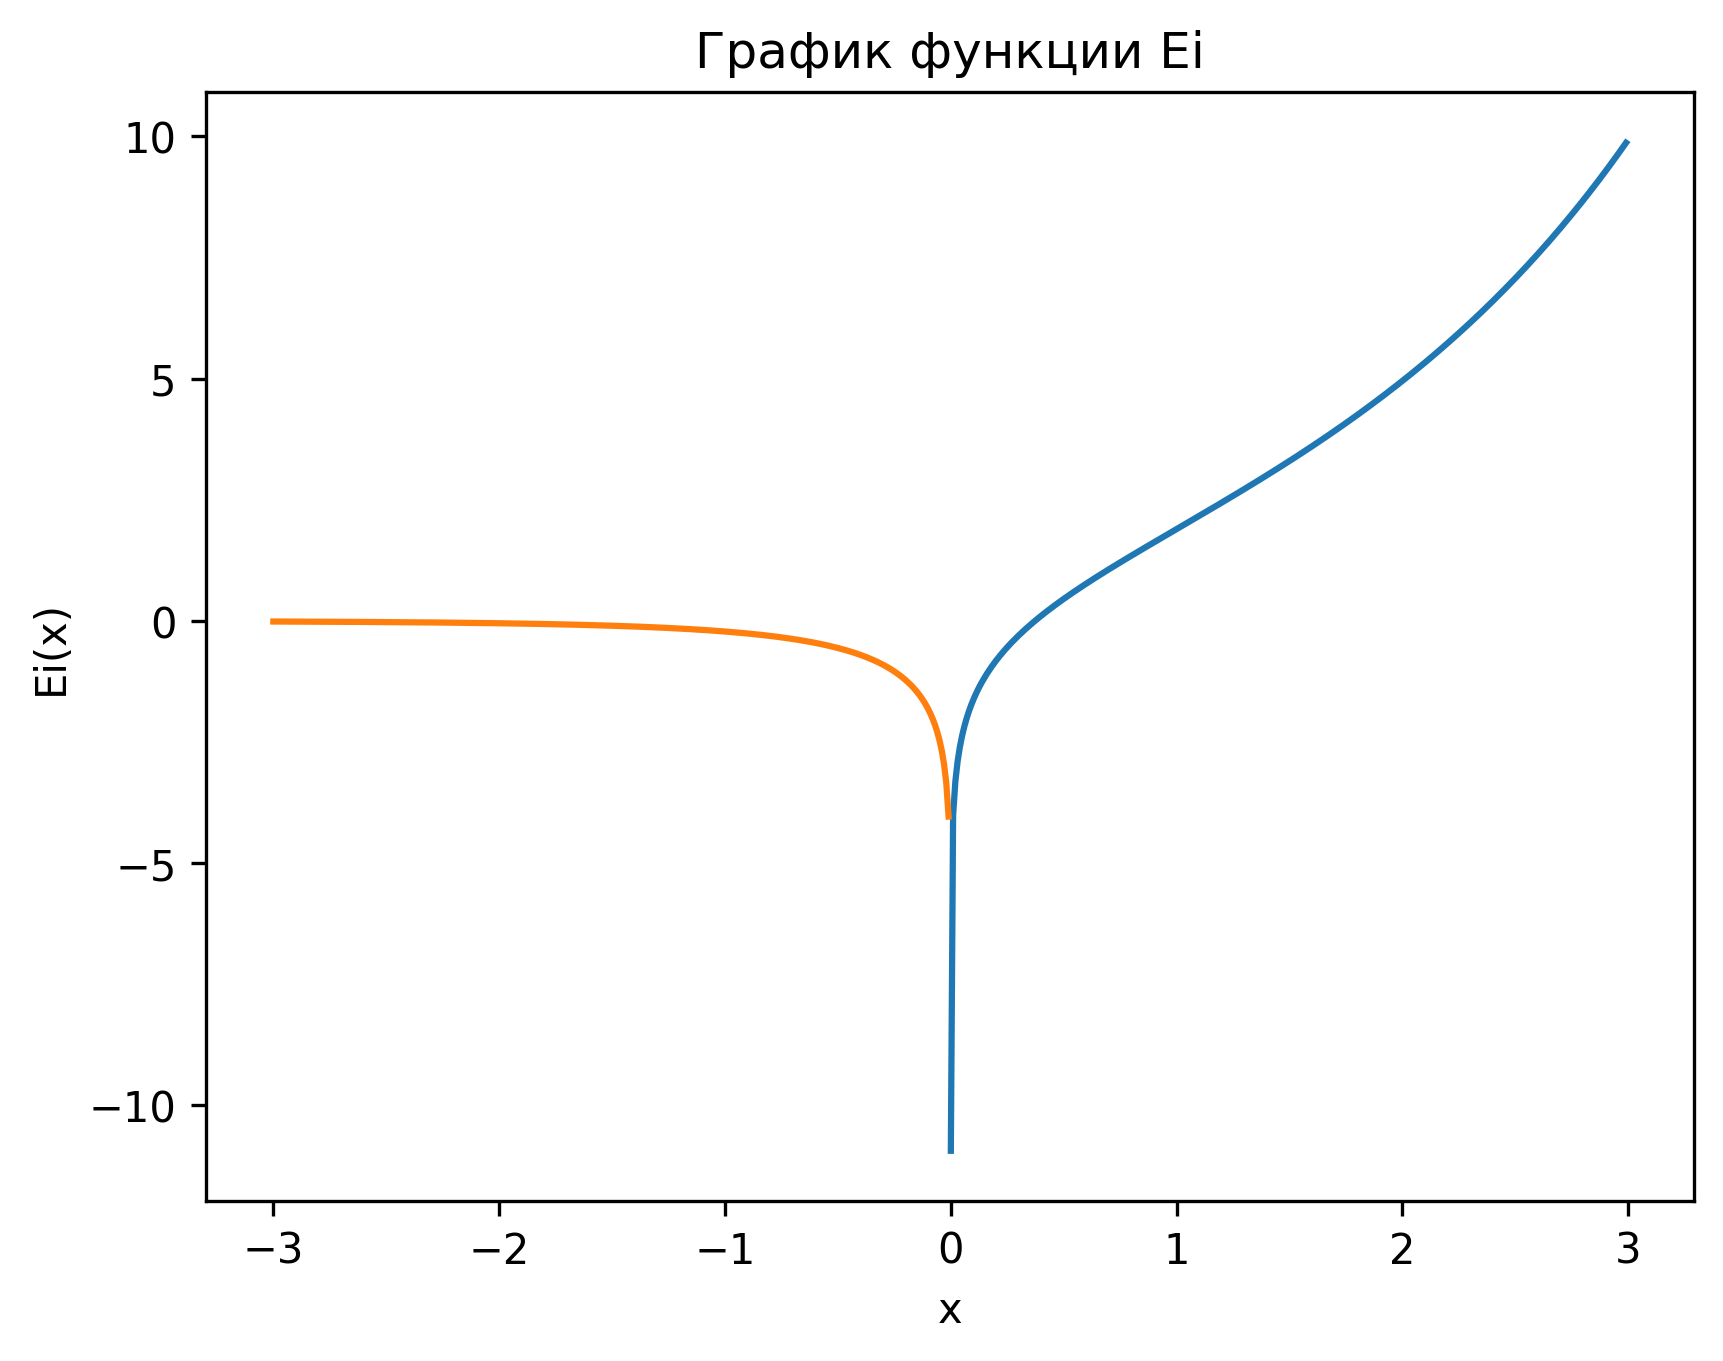
\includegraphics[width=12cm]{pics/Ei_plot_1.png}
		\caption{График функции Ei}
		\label{ris:Ei_plot_1}
	\end{center}
\end{figure}

\begin{figure}
	%\begin{figure}[h!]
	\begin{center}
		\begin{tikzpicture}
			\begin{axis}
				[axis lines = left,
				 width = 0.98\textwidth,
				%xlabel=$x$,
				%ylabel={$Ei_1(x)$},
				]
				\addplot gnuplot[no markers, samples=100, domain = 0:10]{expint(1,x)};
				\addlegendentry{$Ei_1(x)$}
			\end{axis}
		\end{tikzpicture}
		\caption{График функции интегральной экспоненты $Ei_1(x)$.}
		\label{ris:ei1}
	\end{center}
	%\end{figure}
\end{figure}



В этом случае решение может быть выражено через функцию интегральной экспоненты 
\begin{equation}
	p_D(r_D,t_D) = - \frac{1}{2} Ei \left(- \dfrac{ r_D^2}{4t_d} \right)
\end{equation} 

где $-Ei(-x)$ - интегральная показательная функция, рисунок \ref{ris:Ei_plot_1}.

$$Ei(x)=-\int\limits_{x}^{\infty}\frac{e^{-t}}{t}\,\mathrm dt$$

\marginpar{
	\href{https://www.wolframalpha.com/input/?i=Ei\%28x\%29}{$Ei(x)$ Wolfram Alpha} 
	
\includegraphics[scale=0.4]{pics/qr_ei_wolfram.eps} 
	}

Часто для проведения расчетов, особенно с использованием компьютерных библиотеке расчетов, бывает удобнее пользоваться модифицированной интегральной показательной функцией $Ei_1(x)$ или $E_1(x)$ или $Ei_n(x)$ при $n=1$.
 $$Ei_n(x) = \int\limits_{1}^{\infty}\frac{e^{-tx}}{t^n}\,\mathrm dt $$

График интегральной показательной функции $Ei_1(x)$ приведен на рисунке \ref{ris:ei1}.
Для вещественных положительных $x\in\mathbb R, x>0$ верно $E_1(x) = - Ei( -x)$

Функцию интегральной экспоненты можно представить в виде ряда. 

$$Ei(x)=-\int\limits_{x}^{\infty}\frac{e^{-t}}{t}\,\mathrm dt=\gamma+\operatorname{ln}|-x|+\sum\limits_{n\ge1}\frac{{-x}^n}{n!\cdot n}, \;  x\in\mathbb R,\;$$

\begin{figure}
	%\begin{figure}[h!]
	\begin{center}
		\begin{tikzpicture}
			\begin{axis}
				[axis lines = left,
				width = 0.98\textwidth,
				%xlabel=$x$,
				%ylabel={$f(x)$},
				]
				\addplot gnuplot[no markers, samples=100, domain = 0:2]{expint(1,x)};
				\addlegendentry{$Ei_1(x)$}
				\addplot gnuplot[no markers, samples=100, domain = 0:2]{-log(x)-0.5772};
				\addlegendentry{$ln(x)$}
			\end{axis}
		\end{tikzpicture}
		\caption{Сравнение функций интегральной экспоненты $E_1(x)$ и $ln(x)$.}
		\label{ris:ei2}
	\end{center}
	%\end{figure}
\end{figure}

Из приведенного выражения можно сделать выводы, что для маленьких значений аргумента  функция интегральной экспоненты $E_1(x)$ может быть аппроксимирована логарифмической зависимостью. 

$$E_1(x) = -ln(x) - \gamma $$

График сравнения функций $E_1(x)$ и $ln(x)$ показан на рисунке \ref{ris:ei2}. Видно, что хорошей аппроксимация будет только для маленьких значений аргумента $x < 0.01$. Но для решения уравнения фильтрации именно эта зона представляет наибольший интерес.

%\begin{wrapfigure}{r}{0.5\textwidth}
\begin{figure}[h!]
	\begin{center}
		\begin{tikzpicture}
			\begin{axis}
				[axis lines = left,
				width = 0.98\textwidth,
				xlabel=$x$,
				ylabel={$f(x)$},
				xmode=log,
				log ticks with fixed point,
				]
				\addplot gnuplot[no markers, samples=100, domain = 0.00001:20 ]{expint(1,x)};
				\addlegendentry{$Ei_1(x)$}
				\addplot gnuplot[no markers, samples=100, domain = 0.00001:20]{-log(x)-0.5772};
				\addlegendentry{$ln(x)$}
			\end{axis}
		\end{tikzpicture}
		\caption{Сравнение функций интегральной экспоненты $E_1(x)$ и $ln(x)$ в логарифмическом масштабе.Можно оценить диапазон применимости логарифмической аппроксимации.}
		\label{ris:ei3}
	\end{center}
\end{figure}
%\end{wrapfigure}

Представление интегральной экспоненты в виде логарифмической аппроксимации удобно на практике, так как логарифм легче вычислять. В большинстве языков программирования и инструментов для проведения расчетов расчет логарифма реализован по умолчанию. А для расчета интегральной экспоненты, часто приходится предпринимать дополнительные шаги.

Решение уравнения фильтрации для линейного стока с учетом логарифмической аппроксимации можно представить в виде 

\begin{equation}
p_D(r_D,t_D) = \frac{1}{2} \left( ln \left( \dfrac{ t_D }{r_D^2}  \right) +0.809 \right) 
\end{equation}


при использовании данного уравнения, следует помнить, что приближенное решение применимо при $\dfrac{r_D^2}{4t_D} < 0.01$

Решение линейного стока в размерных переменных

\begin{equation}
p\left(r,t\right)=p_i-\frac{18.41q_sB\mu}{kh}\left(-\frac{1}{2}Ei\left(-\frac{\varphi\mu c_tr^2}{0.00144kt}\right)\right) 
\end{equation}

Решение с учетом логарифмической аппроксимации в размерных переменных

\begin{equation}
p\left(r,t\right)=p_i-\frac{9.205q_sB\mu}{kh}\left(ln{\frac{kt}{\varphi\mu c_tr^2}}-7.12\right)
\end{equation}

верно при 
$$\frac{kt}{\varphi\mu c_tr^2}>70000 $$

Решения приведены для практических метрических единиц измерения, что можно увидеть по размерному коэффициенту. 

Нестационарное решение с учетом скин-фактора будет иметь вид


\begin{equation} 
P(r, t) = P_{i} - \frac {9.205 {q_s} B\mu }{k h}(\ ln\frac {k t}{ \varphi \mu {c_t} {r^2}} -7.12 + 2S) 
\end{equation}


%\subsubsection{Радиус исследования}
%Надо бы тут описать концепцию радиуса исследований и подходы к его оценке

\subsubsection{Расчет в Unifloc VBA}

Следующие функции реализованы в Unifloc VBA

\begin{verbatim}
	Ei
	E_1
\end{verbatim}	

Описания функций и из аргументов можно найти в руководстве пользователя  Unifloc VBA



\section{Радиус влияния скважины}


Нестационарное решение в безразмерных переменных
$$ 
p_D(r_D,t_D) = - \frac{1}{2} Ei \left(- \dfrac{ r_D^2}{4t_d} \right)
$$
где безразмерные переменные введены как
$$ r_D = \frac{r}{r_w}  $$
$$ t_D = \frac{0.00036 kt}{\phi \mu c_t r_w^2}  $$
$$ p_D = \frac{kh}{ 18.41 q_s B \mu} \left( p_i - p \right)   $$

Здесь использование единицы измерения СИ.
- $r_w$ - радиус скважины, м

- $r$ - расстояние от центра скважины до точки в пласте, м

- $q_s$ - дебит скважины на поверхности, приведенный к нормальным условиям м3/сут

- $\phi$ - пористость, доли единиц

- $\mu$ - вязкость нефти в пласте, сП

- $B$ - объемный коэффициент нефти, м3/м3

- $p_i$ - начальное давление в пласте, атм

- $p$ - давление на расстоянии $r$, атм

- $c_t$ - общая сжимаемость системы в пласте, 1/атм

Для этих же безразмерных переменных, считая начальное давление равным давлению на контуре можно записать стационарное решение для движения в круговом пласте

$$p_D = \ln r_{eD} - \ln r_D $$

сравним это решение с логарифмической аппроксимацией (1)

$$p_D(r_D,t_D) = - \frac{q_D}{2} \left[ \ln \left( \dfrac{ r_D^2}{4t_d} \right) +\gamma \right] $$

которое можно преобразовать к виду
$$p_D(r_D,t_D) = - q_D \ln r_D  + \frac{q_D}{2} \left[ \ln(4t_D)   -\gamma \right] $$

сравнивая со стационарным решением можно найти выражение безразмерного радиуса контура в зависимости от безразмерного времени
$$\ln r_{eD} = \frac{1}{2}(\ln(4t_D)-\gamma) $$

$$r_{eD} =  \sqrt { 4t_D e^{-\gamma} }  $$

наконец получим
$$r_{eD} = \sqrt {2.2458 t_D} $$

это значение называют радиусом влияния скважины. Используя это значение для определенного момента времени можно получить стационарное распределение давления в системе хорошо приближающее решение линейного стока работающего в бесконечном пласте. Можно считать это расстояние на которое распространяется влияние скважины.

достижение радиуса влияния внешних границ будет обуславливать начало перехода от неустановившегося режима фильтрации к режиму обусловленному влиянием границ - стационарному для границы постоянного давления или псевдо установившемуся для непроницаемой границы.

\begin{figure}[h!]
	\begin{center}
		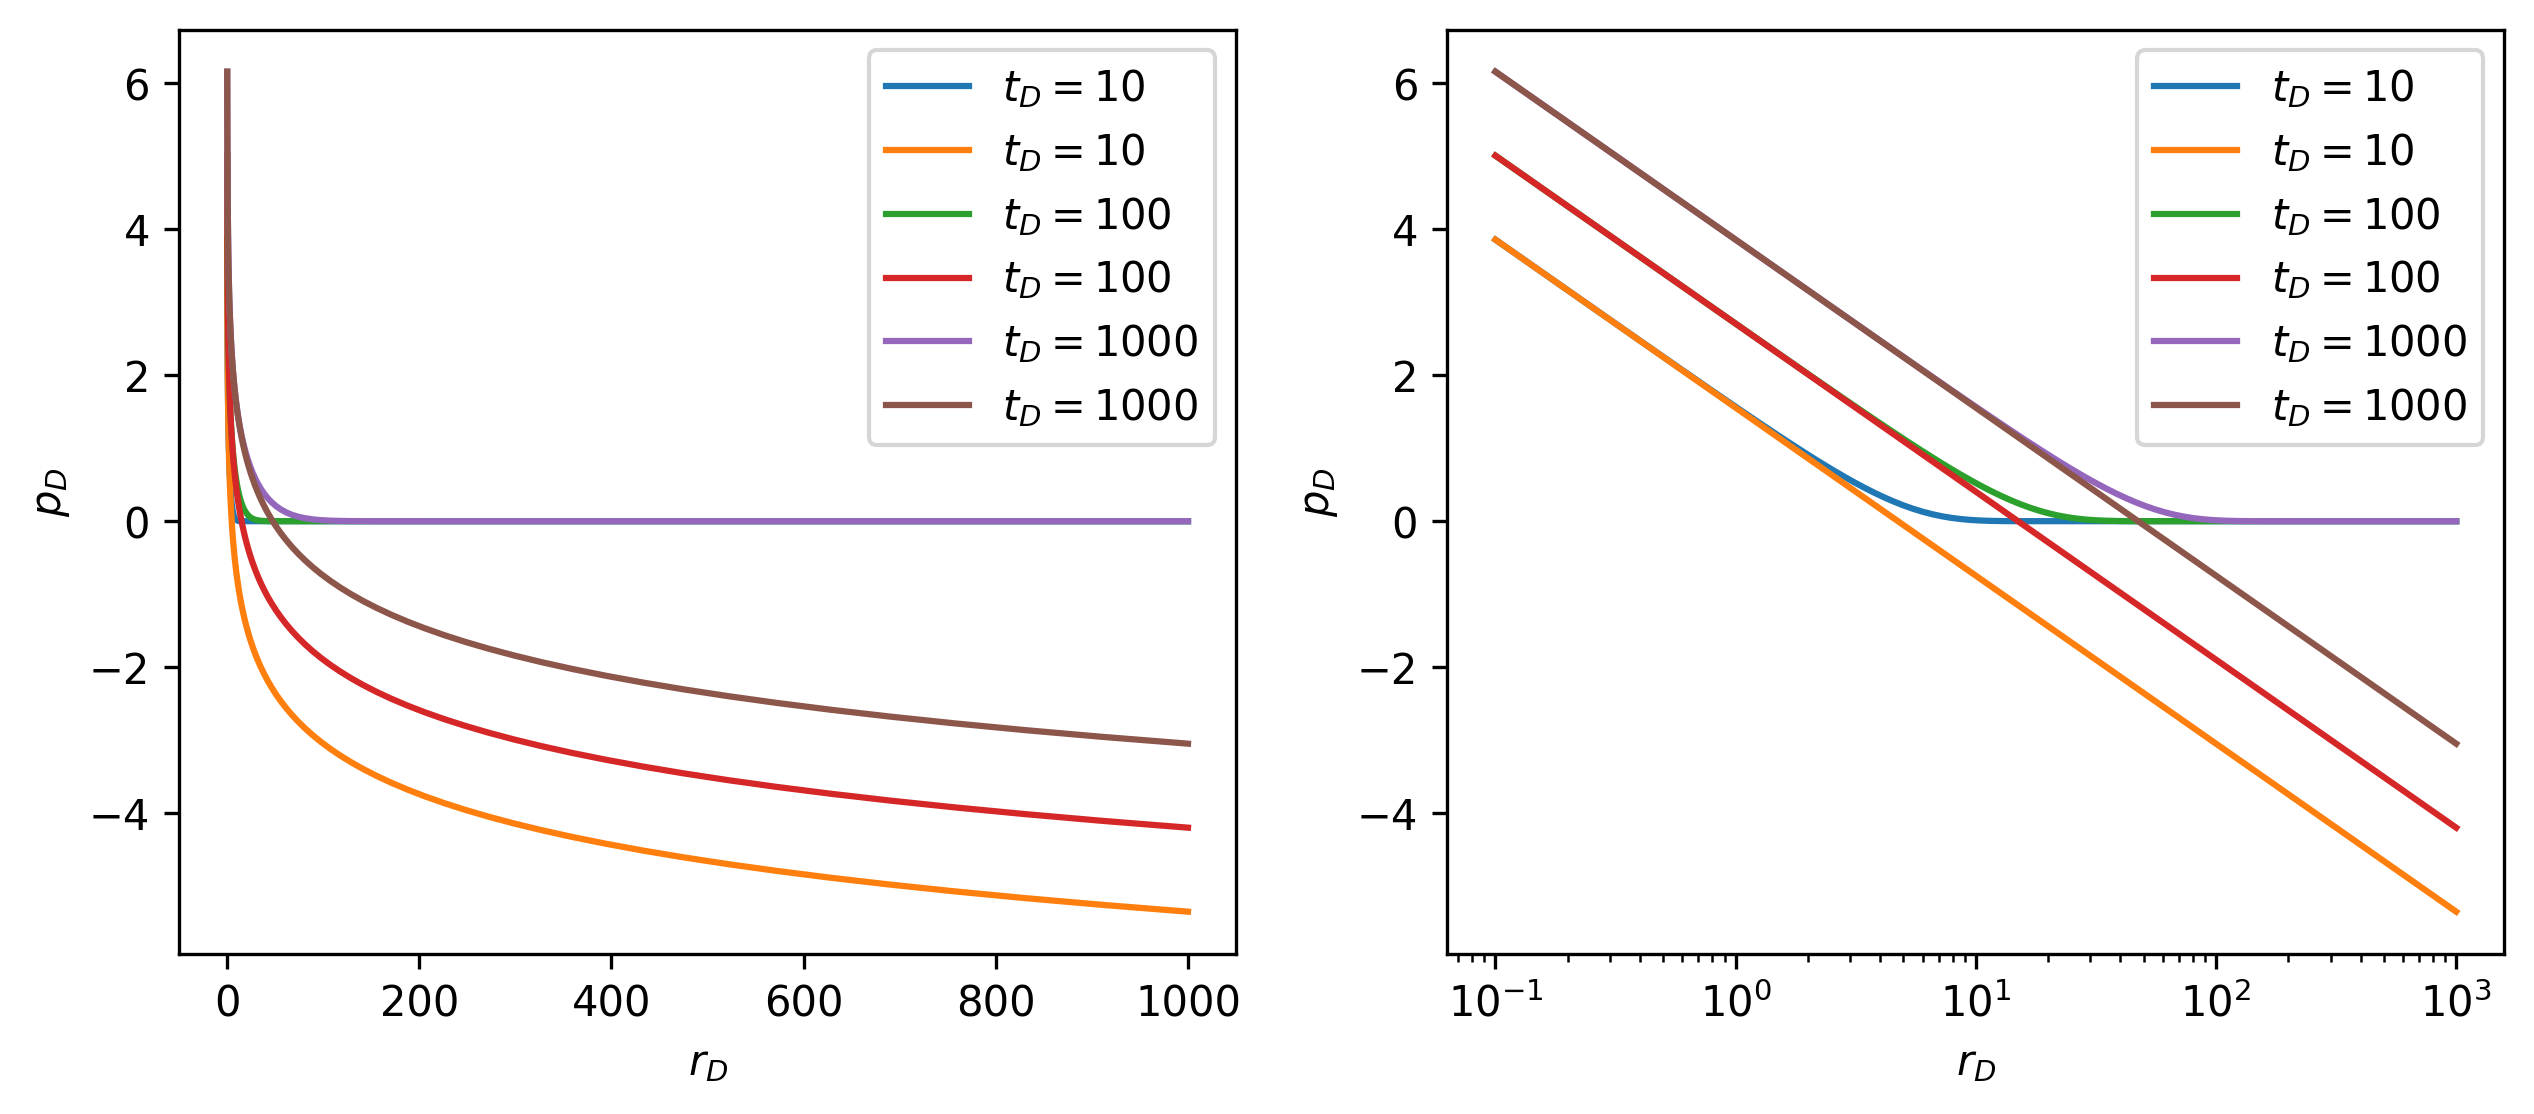
\includegraphics[width=12cm]{pics/stac_radius_investigation_1.png}
		\caption{Изменение радиуса влияния скважины со временем. Сравнение стационарного и нестационарного решений}
		\label{ris:stac_radius_investigation_1}
	\end{center}
\end{figure}




\section{Суперпозиция для нестационарных решений}


Большинство моделей используемых при интерпретации ГДИС основаны на линеаризованном дифференциальном уравнении в частных производных - уравнении фильтрации (уравнении пьезопроводности или диффузии).

$$ \frac{\partial ^2 p }{\partial r^2} + \frac{1}{r} \frac{\partial p}{\partial r} = \frac{\varphi \mu c_t}{k} \frac{\partial p}{\partial t} $$

Для линейных уравнений справедлив принцип суперпозиции - линейная комбинация решений также является решением. То есть если $f(t,r)$ и $g(t,r)$ являются решениями, то $\alpha f(t,r) + \beta g(t,r)$  также является решением.

Это позволяет строить сложные решения уравнения фильтрации на основе простых.

\subsection{Расчет кривой восстановления давления}

Один из самых простых примеров применения суперпозиции. Предполагаем, что добывающая скважина в однородном изотропном пласте запускается в момент времени $t=0$ и работает $t_{p}$ часов, после чего останавливается. После остановки скважины забойное давление растет - и мы получим кривую восстановления давления.

Пусть решение задачи запуска скважины (падения давления) будет $P_D(t_D, r_D)$. Тогда решение для изменения давления при запуске и последующей остановки скважины можно представить в виде 

\begin{equation}
	P_{bu.D}(t_D, t_{prod.D}, r_D) = P_D(t_D) - P_D(t_D-t_{prod.D}, r_D) \cdot \mathcal{H}(t_D-t_{prod.D}) 
\end{equation}

где

- $t_D$ - безразмерное время после запуска скважины,

- $t_{prod.D}$ - безразмерное время работы скважины после запуска

- $\mathcal{H}$ - ступенчатая функция Хевисайда \url{https://ru.wikipedia.org/wiki/Функция_Хевисайда} (в некоторых книгах обозначается как $\theta$)

- $P_D(t_D, r_D)$ - безразмерное давление - решение задачи запуска скважины (падения давления)

- $P_{bu.D}(t_D, t_{prod.D}, r_D)$ - безразмерное давление- решение задачи запуска  и последующей остановки скважины

Для проведения векторных расчетов в python удобно выражение с использованием функции Хевисайда

$$ \mathcal{H} = \begin{cases}0 & x < 0\\1 & x = 0\\1 & x > 0\end{cases}$$

Применение функции Хевисайда позволяет избежать в расчетных функциях условных операторов в явном виде для отдельных элементов входных массивов. Это потенциально ускоряет расчет. 



\subsubsection{Решение для остановки скважины (КВД)}

Для наших целей определим принцип суперпозиции следующим образом: перепад давления в любых точках пласта определяется как сумма перепадов давлений в этих точках, вызванных работой отдельных скважин на залежи. 

Пусть известно решение уравнения фильтрации для запуска скважины с постоянным дебитом в невозмущенном пласте   $p(t)$. 

Известно, что скважина запустилась с дебитом $q$ на период времени $t_p$ и потом остановилась. Требуется найти зависимость изменения давления в скважине после остановки.

$$ p_{D}^{bu}(\Delta t)=p_D(t_p +\Delta t) - p_D(\Delta t)$$  при $\Delta t > 0$

Пример 1.

Рассмотрим случай, когда добывающая скважина работает в различные периоды времени при некоторых постоянных дебитах, как показано на рисунке.  



Итак, рассматривается скважина, работающая с постоянным дебитом $q_1$ в интервале времени от 0 до $t_1$, затем в момент времени $t_1$ дебит изменился и стал равным $q_2$, а при времени $t_2$ дебит вновь изменился и стал равным $q_3$.

Наша задача состоит в определении функции давления на стенке скважины в период времени $t>t_2$.

Для решения этой задачи так же, как и ранее, применим метод суперпозиции, но не в виде учета интерференции соседних скважин, а в виде суммирования дополнительных перепадов давления в самой рассматриваемой скважине:

То есть рассматривается работа нескольких скважин, находящихся в одной точке, но запущенных в работу в разное время. Решение получено для начального дебита $q_1$, за полученное время $t_n$. В момент времени $t_1$ запускается в работу новая скважина с точным известным месторасположением и начальным дебитом $ \left(q_2 - q_1\right)$,так , что чистый дебит скважины после времени  $t_1$ будет равен  $q_2$.В момент времени $t_2$ запускается в работу новая скважина с точным известным месторасположением и начальным дебитом $ \left(q_3 - q_2\right)$, который превращается в дебит $q_3$ после времени $t_2$ …и т. д.

Общее снижение давления в скважине определится с учетом двух изменений дебита притока как:

\begin{eqnarray}
	\left( P_{пл} - P_c\right) = \left( \Delta P\right)_1 + \left( \Delta P\right)_2 +\left( \Delta P\right)_3 = \nonumber  \\ 
	= - \frac{q_1 \mu}{4\pi kh} \left( ln \frac{1,78 \mu m c_t r_c^2}{kt}-2S \right) - \nonumber  \\ 
	\frac{ \left(q_2 - q_1\right)\mu}{4\pi kh} \left( ln \frac{1,78 \mu m c_t r_c^2}{k\left(t-t_1\right)}-2S \right)- \nonumber  \\ 
	\frac{ \left(q_3 - q_2\right)\mu}{4\pi kh} \left( ln \frac{1,78 \mu m c_t r_c^2}{k\left(t-t_2\right)}-2S \right)
\end{eqnarray}

\subsection{Решение для произвольной истории дебитов (ступенчатое изменение дебита)} 

Для расчета изменения давления при переменном дебите введем произвольное референсное значение дебита $ q_{ref} $ (например первое не нулевое значение дебита при запуске скважины). Используем это значение для определения безразмерного давления.
$$ p_D = \frac{kh}{ 18.41 q_{ref} B \mu} \left( p_i - p \right) $$

и безразмерного дебита 

$$q_D = \frac{q}{q_{ref}} $$

Тогда, используя принцип суперпозиции, можем выписать выражение для изменения давления на скважине и вокруг нее для произвольного момента времени

\begin{equation}
	P_{mr.D}(t_D, r_D) = \sum_i \left[ q_{D(i)}-q_{D(i-1)} \right] \cdot p_D\left(t_D-t_{D(i)}, r_D\right)\cdot \mathcal{H}(t_D-t_{D(i)}) \tag{7} 
\end{equation}

где

- $i$ - индекс значения дебита в таблице изменения дебитов

- $q_{D(i)}$ - безразмерный дебит с номером $i$, который стартует в момент времени $t_i$. Для первого момента времени $i$ дебит следующий перед ним считается равным нулю

- $t_{D(i)}$ - безразмерный момент времени - включения дебита с номером $i$

- $t_{D}$ - безразмерный момент времени для которого проводится расчет

- $\mathcal{H}$ - ступенчатая функция Хевисайда

- $p_D\left(t\right)$ - зависимость безразмерного давление от времени - решение задачи запуска скважины с постоянным единичным дебитом

- $P_{mr.D} $ - безразмерное давление $P_{mr.D}(t_D, r_D)$ учитывающее историю изменения дебитов скважины

\subsection{Случай для произвольной истории дебитов (линейное изменение дебита)}

для линейно меняющегося дебита $dq_D t_D$ решение можно представить как интеграл

$$
p_D = \int_0^{t_D}{- \frac{dq_D}{2} Ei \left(- \dfrac{ r_D^2}{4t_d} \right) dt_D}
$$



Для линейно меняющегося дебита во времени (как и для любой другой зависимости) надо решение проинтегрировать по времени (надо бы подробнее расписать - сделать это позже, например как у Щелкачева в основах нестационарной фильтрации на стр 321).

Для линейной зависимости дебита от времени 
$$
Q_D = dQ_D \cdot t_D 
$$
можно получить выражение
$$
p_D(r_D,t_D, dQ_D) =-\frac{dQ_D t_D }{2} \left[ \left( 1+ \frac{r_D^2}{4 t_D} \right) Ei \left(- \dfrac{r_D^2}{4t_D} \right) + e^{-\dfrac{r_D^2}{4t_D}} \right] $$ 

где $dQ_D$ - скорость изменения дебита.

Для таблично заданных дебитов и времен можно оценить 

$$
dQ_{D(i)} = \dfrac{Q_{D(i)}-Q_{D(i-1)}}{t_{D(i)} - t_{D(i-1)} } 
$$

Cравните формулу (11) с формулой (9.68) в книге Щелкачева "Основы неустановившейся фильтрации"

Тогда, используя принцип суперпозиции, можем выписать выражение для изменения давления на скважине и вокруг нее для произвольного момента времени

$$P_{mr.D}(t_D, r_D) = \sum_i  p_D\left(t_D-t_{D(i)}, r_D, dQ_{D(i+1)} - dQ_{D(i)}\right)\cdot \mathcal{H}(t_D-t_{D(i)}) $$

где

- $i$ - индекс значения дебита в таблице изменения дебитов

- $dQ_{D(i)}$ - изменение безразмерного дебита относительно безразмерного времени (14.4) 

- $t_{D(i)}$ - безразмерный момент времени - включения дебита с номером $i$

- $t_{D}$ - безразмерный момент времени для которого проводится расчет

- $\mathcal{H}$ - ступенчатая функция Хевисайда

- $p_D\left(t\right)$ - зависимость безразмерного давление от времени - решение задачи запуска скважины с постоянным единичным дебитом

- $P_{mr.D} $ - безразмерное давление $P_{mr.D}(t_D, r_D)$ учитывающее историю изменения дебитов скважины

следует обратить внимание, при суперпозиции скорость изменения дебита вычисляется как $dQ_{D(i+1)} - dQ_{D(i)}$.  при реализации расчета необходимо предусмотреть, чтобы для первого и последнего шага расчет прошел корректно. Для этого можно, например, добавить к массивам дебитов и времени дополнительный значения в начале и в конце массивов соответствующие постоянным значениям дебита. 

Также надо учитывать, что в приведенном выражении массивы должны начинаться со значений $Q_D=0$




